\begin{figure}[htbp]
\centering

% ============ NA�VE-0 BASELINE ============
\begin{subfigure}{\textwidth}
\centering
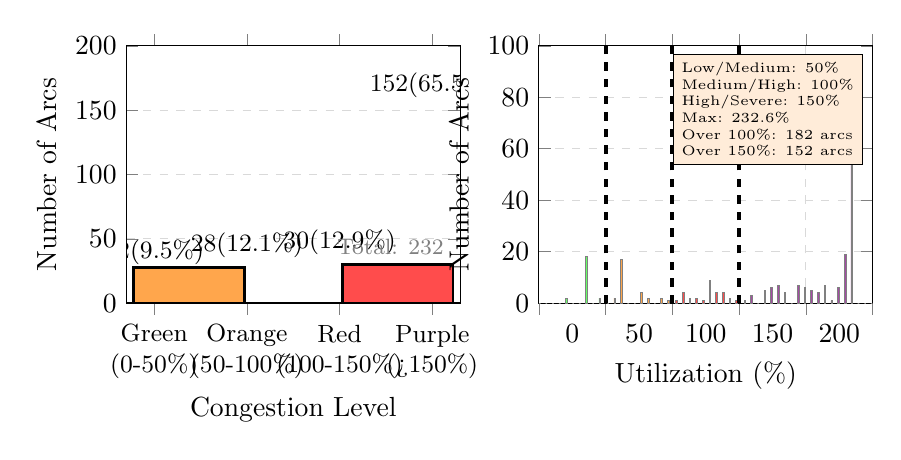
\begin{tikzpicture}

% Left chart - Congestion Level Distribution
\begin{axis}[
    name=left1,
    at={(0,0)},
    width=0.48\textwidth,
    height=0.4\textwidth,
    ybar,
    bar width=40pt,
    xlabel={Congestion Level},
    ylabel={Number of Arcs},
    ymin=0, ymax=200,
    symbolic x coords={Green, Orange, Red, Purple},
    xtick=data,
    xticklabels={Green\\(0-50\%), Orange\\(50-100\%), Red\\(100-150\%), Purple\\(>150\%)},
    x tick label style={align=center, font=\small},
    ymajorgrids=true,
    grid style={dashed, gray!30},
]
\addplot[fill=green!60, draw=black, line width=1pt] coordinates {
    (Green,22) (Orange,0) (Red,0) (Purple,0)
};
\addplot[fill=orange!70, draw=black, line width=1pt] coordinates {
    (Green,0) (Orange,28) (Red,0) (Purple,0)
};
\addplot[fill=red!70, draw=black, line width=1pt] coordinates {
    (Green,0) (Orange,0) (Red,30) (Purple,0)
};
\addplot[fill=violet!70, draw=black, line width=1pt] coordinates {
    (Green,0) (Orange,0) (Red,0) (Purple,152)
};

\node at (axis cs:Green,22) [above, font=\small] {22\\(9.5\%)};
\node at (axis cs:Orange,28) [above, font=\small] {28\\(12.1\%)};
\node at (axis cs:Red,30) [above, font=\small] {30\\(12.9\%)};
\node at (axis cs:Purple,152) [above, font=\small] {152\\(65.5\%)};

\draw[gray, dotted, line width=1.5pt] (axis cs:Green,232) -- (axis cs:Purple,232);
\node[anchor=south east, font=\footnotesize, gray] at (rel axis cs:0.98,0.15) {Total: 232};
\end{axis}

% Right chart - Utilization Histogram
\begin{axis}[
    at={(left1.east)}, anchor=west, xshift=1cm,
    width=0.48\textwidth,
    height=0.4\textwidth,
    ybar interval,
    xlabel={Utilization (\%)},
    ylabel={Number of Arcs},
    xmin=0, xmax=250,
    ymin=0, ymax=100,
    xtick={0,50,100,150,200,250},
    ymajorgrids=true,
    grid style={dashed, gray!30},
]

\addplot[fill=green!60, draw=black!50, line width=0.3pt] coordinates {
    (0,0)
    (5,0)
    (10,0)
    (15,0)
    (20,2)
    (25,0)
    (30,0)
    (35,18)
    (40,0)
    (45,2)
    (50,0)
};
\addplot[fill=orange!70, draw=black!50, line width=0.3pt] coordinates {
    (50,0)
    (55,2)
    (60,17)
    (65,0)
    (70,0)
    (75,4)
    (80,2)
    (85,0)
    (90,2)
    (95,1)
    (100,0)
};
\addplot[fill=red!70, draw=black!50, line width=0.3pt] coordinates {
    (100,1)
    (105,4)
    (110,2)
    (115,2)
    (120,1)
    (125,9)
    (130,4)
    (135,4)
    (140,2)
    (145,1)
    (150,0)
};
\addplot[fill=violet!70, draw=black!50, line width=0.3pt] coordinates {
    (150,1)
    (155,3)
    (160,0)
    (165,5)
    (170,6)
    (175,7)
    (180,4)
    (185,0)
    (190,7)
    (195,6)
    (200,5)
    (205,4)
    (210,7)
    (215,1)
    (220,6)
    (225,19)
    (230,71)
    (235,0)
    (240,0)
    (245,0)
    (250,0)
};

\draw[black, dashed, line width=1.5pt] (axis cs:50,0) -- (axis cs:50,100);
\draw[black, dashed, line width=1.5pt] (axis cs:100,0) -- (axis cs:100,100);
\draw[black, dashed, line width=1.5pt] (axis cs:150,0) -- (axis cs:150,100);

\node[anchor=north east, font=\tiny, align=left, fill=orange!15, draw=black, inner sep=3pt]
    at (rel axis cs:0.97,0.97) {
    Low/Medium: 50\%\\
    Medium/High: 100\%\\
    High/Severe: 150\%\\
    Max: 232.6\%\\
    Over 100\%: 182 arcs\\
    Over 150\%: 152 arcs
};
\end{axis}
\end{tikzpicture}
\caption{Na�ve-0 baseline (Mean util: 169.0\%, Median: 195.2\%)}
\end{subfigure}

\vspace{0.8cm}

% ============ RANDOM BASELINE ============
\begin{subfigure}{\textwidth}
\centering
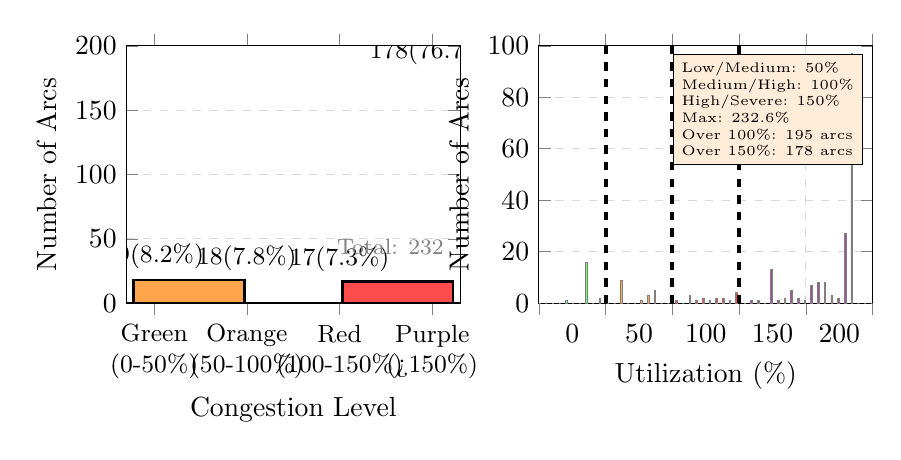
\begin{tikzpicture}

% Left chart - Congestion Level Distribution
\begin{axis}[
    name=left2,
    at={(0,0)},
    width=0.48\textwidth,
    height=0.4\textwidth,
    ybar,
    bar width=40pt,
    xlabel={Congestion Level},
    ylabel={Number of Arcs},
    ymin=0, ymax=200,
    symbolic x coords={Green, Orange, Red, Purple},
    xtick=data,
    xticklabels={Green\\(0-50\%), Orange\\(50-100\%), Red\\(100-150\%), Purple\\(>150\%)},
    x tick label style={align=center, font=\small},
    ymajorgrids=true,
    grid style={dashed, gray!30},
]
\addplot[fill=green!60, draw=black, line width=1pt] coordinates {
    (Green,19) (Orange,0) (Red,0) (Purple,0)
};
\addplot[fill=orange!70, draw=black, line width=1pt] coordinates {
    (Green,0) (Orange,18) (Red,0) (Purple,0)
};
\addplot[fill=red!70, draw=black, line width=1pt] coordinates {
    (Green,0) (Orange,0) (Red,17) (Purple,0)
};
\addplot[fill=violet!70, draw=black, line width=1pt] coordinates {
    (Green,0) (Orange,0) (Red,0) (Purple,178)
};

\node at (axis cs:Green,19) [above, font=\small] {19\\(8.2\%)};
\node at (axis cs:Orange,18) [above, font=\small] {18\\(7.8\%)};
\node at (axis cs:Red,17) [above, font=\small] {17\\(7.3\%)};
\node at (axis cs:Purple,178) [above, font=\small] {178\\(76.7\%)};

\draw[gray, dotted, line width=1.5pt] (axis cs:Green,232) -- (axis cs:Purple,232);
\node[anchor=south east, font=\footnotesize, gray] at (rel axis cs:0.98,0.15) {Total: 232};
\end{axis}

% Right chart - Utilization Histogram
\begin{axis}[
    at={(left2.east)}, anchor=west, xshift=1cm,
    width=0.48\textwidth,
    height=0.4\textwidth,
    ybar interval,
    xlabel={Utilization (\%)},
    ylabel={Number of Arcs},
    xmin=0, xmax=250,
    ymin=0, ymax=100,
    xtick={0,50,100,150,200,250},
    ymajorgrids=true,
    grid style={dashed, gray!30},
]

\addplot[fill=green!60, draw=black!50, line width=0.3pt] coordinates {
    (0,0)
    (5,0)
    (10,0)
    (15,0)
    (20,1)
    (25,0)
    (30,0)
    (35,16)
    (40,0)
    (45,2)
    (50,0)
};
\addplot[fill=orange!70, draw=black!50, line width=0.3pt] coordinates {
    (50,0)
    (55,0)
    (60,9)
    (65,0)
    (70,0)
    (75,1)
    (80,3)
    (85,5)
    (90,0)
    (95,0)
    (100,0)
};
\addplot[fill=red!70, draw=black!50, line width=0.3pt] coordinates {
    (100,1)
    (105,0)
    (110,3)
    (115,1)
    (120,2)
    (125,1)
    (130,2)
    (135,2)
    (140,1)
    (145,4)
    (150,0)
};
\addplot[fill=violet!70, draw=black!50, line width=0.3pt] coordinates {
    (150,0)
    (155,1)
    (160,1)
    (165,0)
    (170,13)
    (175,1)
    (180,2)
    (185,5)
    (190,2)
    (195,1)
    (200,7)
    (205,8)
    (210,8)
    (215,3)
    (220,2)
    (225,27)
    (230,97)
    (235,0)
    (240,0)
    (245,0)
    (250,0)
};

\draw[black, dashed, line width=1.5pt] (axis cs:50,0) -- (axis cs:50,100);
\draw[black, dashed, line width=1.5pt] (axis cs:100,0) -- (axis cs:100,100);
\draw[black, dashed, line width=1.5pt] (axis cs:150,0) -- (axis cs:150,100);

\node[anchor=north east, font=\tiny, align=left, fill=orange!15, draw=black, inner sep=3pt]
    at (rel axis cs:0.97,0.97) {
    Low/Medium: 50\%\\
    Medium/High: 100\%\\
    High/Severe: 150\%\\
    Max: 232.6\%\\
    Over 100\%: 195 arcs\\
    Over 150\%: 178 arcs
};
\end{axis}
\end{tikzpicture}
\caption{Random baseline (Mean util: 187.2\%, Median: 229.0\%)}
\end{subfigure}

\vspace{0.8cm}

% ============ OPTIMIZATION ============
\begin{subfigure}{\textwidth}
\centering
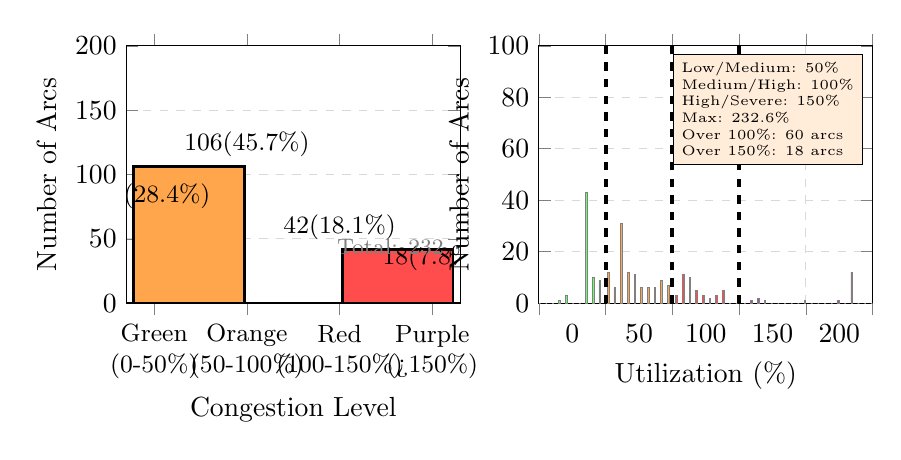
\begin{tikzpicture}

% Left chart - Congestion Level Distribution
\begin{axis}[
    name=left3,
    at={(0,0)},
    width=0.48\textwidth,
    height=0.4\textwidth,
    ybar,
    bar width=40pt,
    xlabel={Congestion Level},
    ylabel={Number of Arcs},
    ymin=0, ymax=200,
    symbolic x coords={Green, Orange, Red, Purple},
    xtick=data,
    xticklabels={Green\\(0-50\%), Orange\\(50-100\%), Red\\(100-150\%), Purple\\(>150\%)},
    x tick label style={align=center, font=\small},
    ymajorgrids=true,
    grid style={dashed, gray!30},
]
\addplot[fill=green!60, draw=black, line width=1pt] coordinates {
    (Green,66) (Orange,0) (Red,0) (Purple,0)
};
\addplot[fill=orange!70, draw=black, line width=1pt] coordinates {
    (Green,0) (Orange,106) (Red,0) (Purple,0)
};
\addplot[fill=red!70, draw=black, line width=1pt] coordinates {
    (Green,0) (Orange,0) (Red,42) (Purple,0)
};
\addplot[fill=violet!70, draw=black, line width=1pt] coordinates {
    (Green,0) (Orange,0) (Red,0) (Purple,18)
};

\node at (axis cs:Green,66) [above, font=\small] {66\\(28.4\%)};
\node at (axis cs:Orange,106) [above, font=\small] {106\\(45.7\%)};
\node at (axis cs:Red,42) [above, font=\small] {42\\(18.1\%)};
\node at (axis cs:Purple,18) [above, font=\small] {18\\(7.8\%)};

\draw[gray, dotted, line width=1.5pt] (axis cs:Green,232) -- (axis cs:Purple,232);
\node[anchor=south east, font=\footnotesize, gray] at (rel axis cs:0.98,0.15) {Total: 232};
\end{axis}

% Right chart - Utilization Histogram
\begin{axis}[
    at={(left3.east)}, anchor=west, xshift=1cm,
    width=0.48\textwidth,
    height=0.4\textwidth,
    ybar interval,
    xlabel={Utilization (\%)},
    ylabel={Number of Arcs},
    xmin=0, xmax=250,
    ymin=0, ymax=100,
    xtick={0,50,100,150,200,250},
    ymajorgrids=true,
    grid style={dashed, gray!30},
]

\addplot[fill=green!60, draw=black!50, line width=0.3pt] coordinates {
    (0,0)
    (5,0)
    (10,0)
    (15,1)
    (20,3)
    (25,0)
    (30,0)
    (35,43)
    (40,10)
    (45,9)
    (50,0)
};
\addplot[fill=orange!70, draw=black!50, line width=0.3pt] coordinates {
    (50,12)
    (55,6)
    (60,31)
    (65,12)
    (70,11)
    (75,6)
    (80,6)
    (85,6)
    (90,9)
    (95,7)
    (100,0)
};
\addplot[fill=red!70, draw=black!50, line width=0.3pt] coordinates {
    (100,3)
    (105,11)
    (110,10)
    (115,5)
    (120,3)
    (125,2)
    (130,3)
    (135,5)
    (140,0)
    (145,0)
    (150,0)
};
\addplot[fill=violet!70, draw=black!50, line width=0.3pt] coordinates {
    (150,0)
    (155,1)
    (160,2)
    (165,1)
    (170,0)
    (175,0)
    (180,0)
    (185,0)
    (190,0)
    (195,1)
    (200,0)
    (205,0)
    (210,0)
    (215,0)
    (220,1)
    (225,0)
    (230,12)
    (235,0)
    (240,0)
    (245,0)
    (250,0)
};

\draw[black, dashed, line width=1.5pt] (axis cs:50,0) -- (axis cs:50,100);
\draw[black, dashed, line width=1.5pt] (axis cs:100,0) -- (axis cs:100,100);
\draw[black, dashed, line width=1.5pt] (axis cs:150,0) -- (axis cs:150,100);

\node[anchor=north east, font=\tiny, align=left, fill=orange!15, draw=black, inner sep=3pt]
    at (rel axis cs:0.97,0.97) {
    Low/Medium: 50\%\\
    Medium/High: 100\%\\
    High/Severe: 150\%\\
    Max: 232.6\%\\
    Over 100\%: 60 arcs\\
    Over 150\%: 18 arcs
};
\end{axis}
\end{tikzpicture}
\caption{Optimization (Mean util: 81.1\%, Median: 65.1\%)}
\end{subfigure}

\caption{Arc utilization statistics for the 250 ID trip instance (medium traffic). Left panels show congestion level distribution. Right panels show detailed utilization histograms with 5\% bins and dashed vertical lines marking congestion thresholds. The optimization achieves dramatically better distribution: only 60 arcs exceed 100\% utilization (vs 195 for Na�ve, 182 for Random) and just 18 arcs exceed 150\% (vs 178 for Na�ve, 152 for Random).}
\label{fig:utilization_comparison}
\end{figure}